% Introdução: cenario, motivacao, problema, solucoes atuais, escopo do trabalho, lista de contribuicoes, organizacao do resto do artigo. 
% Chapter Structure
% 	Motivation
% 	Problems Statement
%	Contributions
% 	Dissertation Organization
\chapter{Introduction}
\label{ch:1_introduction}

According to Gartner surveys and client feedback, security remains a top concern for business and IT leaders. Cybersecurity is also highly visible in the media because of privacy concerns, destructive attacks such as ransomware, fears around IoT hacking, and an increasingly visible effect of cybersecurity on geopolitics \cite{Chuvakin2018}.

The Whitehouse of the U.S. government \cite{whitehouse2018} estimates that malicious cyber activity cost the U.S. economy between US\$57 billion and US\$109 billion in 2016. According to Bissel \emph{et al.} \cite{BISSELL2019}, the total annual cost of all types of cyberattacks is increasing. Malware and Web-based attacks continue to be the most expensive threats for global companies, corresponding to US\$2.6 million and US\$2.2 million, respectively. However, it is possible to observe an increasing of 10\% of Denial of Service (DoS) attack, 12\% of botnets, 15\% of malicious insider and an increment of 21\% in occurrences of ransomware, between 2017 and 2018 \cite{BISSELL2019}.

Accenture's study conducted by Bissel \emph{et al.} \cite{BISSELL2019} shows that the extent of the economic value may be at risk if security investments are not made wisely. Bissel \emph{et al.} \cite{BISSELL2019} shows that the size of opportunity varies by industry, with high tech subject to the greatest value at risk — US\$753 billion — over the next five years, followed by US\$ 642 billion for life sciences and US\$505 billion for the automotive industry. Bissel \emph{et al.} \cite{BISSELL2019} analyze the total technology savings minus total technology spend in cybersecurity by organizations, reporting that security intelligence and threat sharing have been adopted by 67\% of respondents and saving US\$2.26 million. Bissel \emph{et al.} \cite{BISSELL2019} also reported that automation, artificial intelligence, and machine learning have been adopted by 38\% of respondents and saving US\$2.09 million, while the cyber and user behavior analytics have been adopted by 32\% of respondents and saving US\$1.72 million.

Additionally, Levi \cite{Levi2019} highlights that Blizzard Entertainment was hit by a Distributed Denial of Service (DDoS) attack in 2017, when the downtime lasted an entire weekend, due to difficulties related to track the root cause of the anomaly. According to Levi \cite{Levi2019}, attacks like these can cost an enterprise more than US\$2 million, which makes anomaly detection essential to protecting revenue.

Traditionally, cyber defense methods can be effective against well-known types of attacks, yet may fail against innovative malicious techniques \cite{lakhina2005mining}. In order to be able to detect and avoid network attacks and their variations, it is necessary to develop or improve techniques to achieve efficiency in resource consumption, processing capacity and response time. Moreover, it is crucial to obtain high detection accuracy and capacity to detect variations of malicious patterns. Several efforts and researches aim to avoid network attacks based on known attackers, fingerprints or behavioral analysis \cite{gu2008botminer, khattak2015botflex}. 

An attacker can create a bot for malicious purposes to generate a DoS attack, to exploit or abuse a target application. A botnet is a collection of bots or systems for executing automated tasks, often in the form of compromised hosts, including desktops, mobile devices or things (as in IoT). Some recent common examples of botnets include Cyclone, Mirai, Nitol and Sentry MBA \cite{Catucci2019}. Distributed attacks organized by botnet has increased and demanded the development of counter measures, in order to detect and avoid unknown attacks or even to deal with adversarial changes of behavior, location and other patterns \cite{wang2017botnet, Wang2018ddosbotnetssurvey}.

According to Hevesi \cite{Hevesi2019} in a Gartner's publication, Botnets scan the Internet looking for unprotected Internet of Things (IoT) devices — and there are projected to be 25 billion devices online in 2021. Mobile network providers are deploying 5G capabilities to their networks, and industry is looking for new ways to leverage the service to bring new capabilities to market. Hevesi argues that if just 1\% was able to be added to a botnet and had access to 5G, the potential network throughput would be 250 million devices able to push 10 to 50 Gbps of network traffic in a flooding attack.

Cyber security systems can work in the following fashions: signature-based, anomaly-based or hybrid \cite{mudzingwa2012study}. A signature or fingerprint can be seen as a sequence of data, behavior and rules which are often unique to known malware or attack types, allowing the identification of attackers that reproduce some signature, such as occurs in less sophisticated viruses and automated toolkits for security exploitation and intrusion. However, signature-based systems for attack detection have to deal with adversarial models and techniques that aims to avoid detection based on well-known patterns, such as instruction virtualization, packing, polymorphism, emulation, and metamorphism to write and change malicious codes that can evade the detection \cite{bhuyan2014network}.

Anomaly-based systems for network attack detection focus on finding exceptional, suspicious or rare observations in network traffic that do not conform to the expected legitimate behavior \cite{bhuyan2014network}. In a general view, anomalies are referred to as outliers, novelties or deviations, and can be related to defects, diseases, network attacks, intrusion detection for cyber security, fraud detection for credit cards, and military surveillance issues. Additionally, anomaly detection techniques can be categorized by classification, statistical algorithms, information theory and cluster based algorithms, according to \cite{ahmed2016survey}. 

Hybrid systems for network attack detection exploit benefits of both signature-based and anomaly-based detection techniques, and attempt to detect known as well as unknown attacks \cite{ahmed2016survey}.

%Recent developments in science and technology have enabled the growth and availability of raw data to occur at an explosive rate. This has created an immense opportunity for knowledge discovery and data engineering research to play an essential role in a wide range of applications from daily civilian life to national security. Despite the high availability of information, the relevant information for network anomaly detection from the whole network traffic is lower than the total available traffic, with very imbalanced classes and with susceptibility to imbalanced learning problem.

Accenture consulting argues that 89\% of survey respondents believe breakthrough technologies, like artificial intelligence, machine or deep learning, user behavior analytics, and blockchain, are essential for securing the future of their organizations \cite{Accenture2018}. To face the adversarial model, novel attacks and counter measures of attackers to avoid detection, it is possible to adopt unsupervised or semi-supervised approaches for network anomaly detection, by means of behavioral analysis, where known anomalies are not necessaries for training models \cite{moustafa2019holistic}. 

Recently, signal processing schemes have been applied to detect malicious traffic in computer networks by means of unsupervised approaches, showing advances in network traffic analysis \cite{Zonglin2009}, in network attack detection \cite{callegari2011novel}, and in network anomaly detection based on network flows \cite{Lu2009}. 

Furthermore, it is possible to observe that anomaly-based and behavioral-based solutions have been adopted for cyber security and attracting investments, as can be seen in the Featurespace case, which is a provider of adaptive behavioral analytics for fraud detection and risk management, that raised US\$32.3 million from a funding round led by Insight Venture Partners and MissionOG \cite{Williams2019}.

Anomalies in the context of network traffic can be hard to identify and separate from legitimate data due to the rare occurrences of anomalies in comparison to legitimate events. Therefore, anomaly detection algorithms have to be highly discriminating, robust to corruption and able to deal with the imbalanced data problem \cite{he2008learning}. Note that data corruption refers to outliers that can be part of the data, while the imbalanced data problem corresponds to data sets exhibiting significant imbalances of classes or rare events of some classes \cite{he2009learning}, which can be legitimate or malicious classes in network anomaly detection problems. 

The imbalanced data can compromise the performance of most standard learning algorithms, creating bias or unfair weight to learn from the majority class and reducing detection capacity of anomalies that are characterized by the minority class. Hence, data analysis of imbalanced data is challenging for learning algorithms applied to classification problems of anomaly detection, novelty detection, fraud detection and network attack detection. However, anomaly-based algorithms, that rely on unsupervised or semi-supervised approaches, can be alternatives for network anomaly detection from imbalanced data \cite{moustafa2019holistic}.

Some widely adopted algorithms for anomaly detection assume a Gaussian distributed legitimate data \cite{lakhina2005mining}, however this assumption may not be observed in real world problems, such as the case of network traffic analysis \cite{benson2010network}, where network traffic features are usually more characterized by skewed and heavy-tailed distributions \cite{benson2010network, leon2017probability}. According to \cite{hubert2009robustskewed}, the skeweness and heavy-tailed distributions can impact algorithms that rely on Gaussian distributed data, and can reveal characteristics that can be exploited in order to obtain accurate classifiers for network anomaly detection.

Therefore, this thesis focus on anomaly-based problems. More specifically, we focus on network attack detection and propose behavioral-based approaches for network anomaly detection through subspace learning techniques and similarity analysis. 

Firstly, we propose the Eigensimilarity, which is an approach based on signal processing methods applied to detection of probe and flooding attacks in computer networks. We present an architecture and approach to evaluate a proof of concept of Eigensimilarity for malicious behavior detection on mobile applications, in order to detect possible threats in offline corporate mobile client. Additionally, we propose the Moment-based Robust Principal Component Analysis (m-RPCA), which is an approach based on distances between contaminated observations and moments computed from a robust subspace learned by Robust Principal Component Analysis (RPCA), in order to detect anomalies from imbalanced and skewed data, such as network traffic.

This chapter is organized as follows. The problem statement, the hypotheses formulation and the proposed approaches for network attack detection are introduced in Section \ref{sec:1_problems}. In Section \ref{sec:1_contributions} we present the main contributions of this thesis and in Section \ref{sec:1_organization} we describe the thesis organization for the next chapters.

\section{Problem Statement}
\label{sec:1_problems}

Considering the previous described landscape, this thesis outlines the development and evaluation of approaches based on subspace learning for network attack detection, through methods to make the data discriminative and able to identify structures, hidden patterns and the most relevant information for anomaly detection. In Subsection \ref{sec:1_Hypothesis} we present our hypothesis formulation and in Subsection \ref{sec:1_proposals} we describe the proposed approaches to answer the questions and validate the hypotheses.

\subsection{Hypothesis Formulation}
\label{sec:1_Hypothesis}

For the experimental evaluation of our proposals, we adopt a methodology based on aspects of Goal-Question-Metric (GQM) template \citep{Basili1994} and define two questions to achieve our goal, which are:

\begin{itemize}
	\item $Q_1$: Can the analysis of patterns from a learned subspace identify and detect anomalies in network traffic?
	\item $Q_2$: Can the robust subspace learning improve the anomaly detection in imbalanced and skewed data?
\end{itemize}

Our testing hypotheses are defined in Table \ref{tab:hypothesis}, that describe the null hypotheses ($H_1^{(N)}$ and $H_2^{(N)}$) and alternative hypotheses ($H_1^{(A)}$ and $H_2^{(A)}$) for each previously defined question. 

\begin{table}[htb]
	\centering
	\caption{Hypotheses to evaluate the defined questions}
	\label{tab:hypothesis}
    \begin{tabular}{|p{6cm}|p{6cm}|c|} \hline
        \textbf{Alternative Hypothesis}	&\textbf{Null Hypothesis}	&\textbf{Question} 	\\ \hline
        $H_1^{(A)}$: A subspace learned by eigenvalue decomposition can be used to detect and identify network attacks.
        &$H_1^{(N)}$. A subspace learned by eigenvalue decomposition can not be used to detect and identify network attacks.	&$Q_1$\\ \hline
        $H_2^{(A)}$: An approach based on robust subspace learning improves the anomaly detection from imbalanced and skewed data.	&$H_2^{(N)}$. An approach based on robust subspace learning does not improves the anomaly detection from imbalanced and skewed data.	&$Q_2$\\ \hline
    \end{tabular}
\end{table}

The hypotheses $H_1^{(A)}$ and $H_1^{(N)}$ are defined to evaluate if a subspace learned by eigenvalue decomposition are sensitive to outliers and can be used to detect network attacks. We define the hypotheses $H_2^{(A)}$ and $H_2^{(N)}$ to evaluate if the distance between contaminated data and robust moments learned by Robust Principal Component Analysis (RPCA) can improve the anomaly detection in simulated imbalanced and skewed data. 

%The metrics most adopted to evaluate experimental results of network attack detection are the true positive (TP), true negative (TN), false positive (FP) and false negative (FN). We adopt these metrics and also adopt the misclassification rate and the F1-score, which is the preferable measure for imbalanced data sets \cite{powers2011evaluation,moustafa2019holistic}.

\subsection{Proposals}
\label{sec:1_proposals}

In the context of anomaly-based schemes, this thesis proposes the Eigensimilarity, which is an approach based on subspace learning techniques for detection of malicious traffic in computer networks, by means of eigenvalue analysis, model order selection (MOS) and a similarity analysis between eigenvectors of estimated legitimate observations and observations of a time frame estimated as under attack.

In contrast to \cite{david2011blind,da2012improved,tenorio2013greatest}, MOS and eigenvalue analysis are applied to detect detailed time frames under attack. We evaluate the accuracy and performance of the proposed framework applied to an experimental scenario and to the DARPA 1998 data set \citep{osanaiye2016distributed}, which is a well-known network traffic data set. Furthermore, this proposed approach is evaluated by a proof of concept regarding behavioral anomaly detection to detect possible threats to an offline corporate mobile app. 

The skewness of anomalous and legitimate data can highlight features for improving anomaly detection in imbalanced data, and the distance between robust estimates of legitimate observations and contaminated data can be used for network attack detection. Therefore, we propose the Moment-based Robust Principal Component Analysis (m-RPCA), which is an approach based on distances of moments computed from a robust subspace learned by RPCA, for anomaly detection on imbalanced and skewed data. We evaluate the results of m-RPCA for anomaly detection on simulated imbalanced and skewed data, and evaluate the results of m-RPCA for network attack detection on CTU-13 data set.

Eigensimilarity and m-RPCA are frameworks for network attack detection by means of anomaly-based analysis from network traffic. In a simplified architecture for network attack detection shown by Figure \ref{fig:1.01}, Eigensimilarity and m-RPCA are deployed as a module of an application firewall, which is responsible for secure and protect application communications, but can also work on network level. 

\begin{figure}[h!]
	\centering
     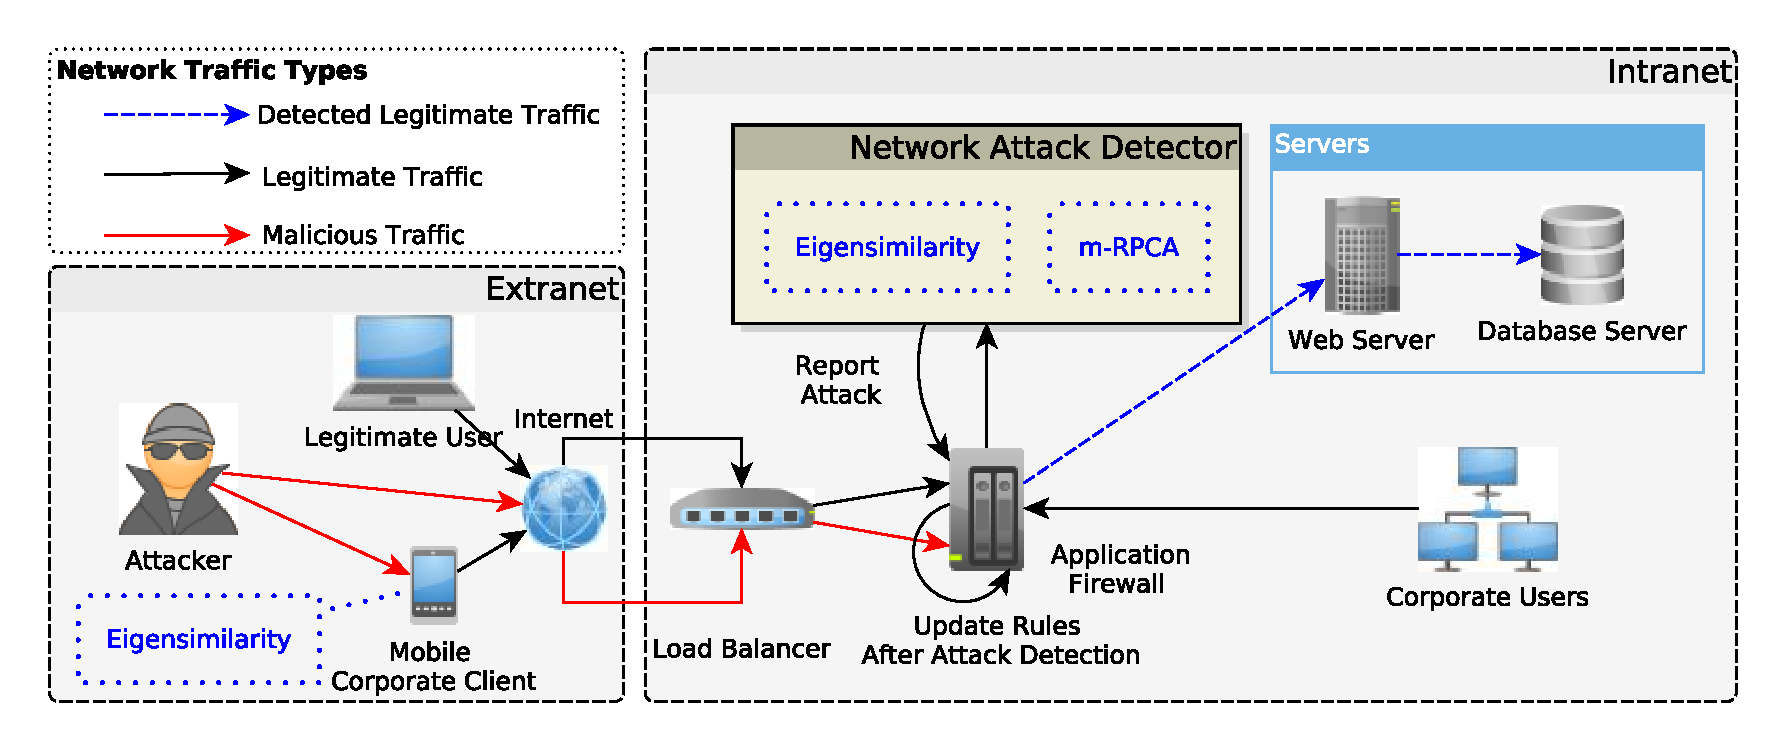
\includegraphics[width=15cm]{figures/ch1/architecture.eps} 
     \caption{Simplified Architecture for Network Attack Detection.}
     \label{fig:1.01}
\end{figure}

An application firewall can implement behavioral analysis in order to detect attacks against application services, such as Spam or Click Fraud (CF), or can detect anomalies in network level, such as a DoS attack based on Ping flood.

The Figure \ref{fig:1.01} depicts the flow of network traffic between legitimate or malicious users to a corporate network. All income traffic shall be received and distributed by the load balancer, to be evaluated by an application firewall, which is is responsible for network attack detection. Therefore, the application firewall implements a high throughput traffic analyzer, to capture and parse the network traffic for further analysis, by means of Eigensimilarity and m-RPCA. The Figure \ref{fig:1.01} also depicts the use of Eigensimilarity as a module of an offline corporate mobile app, as a proof of concept regarding behavioral anomaly detection from user activities.


\section{Contributions}
\label{sec:1_contributions}

We analyze problems related to detection of information security issues in network traffic and propose new approaches to improve malicious behavior detection through signal processing techniques based on subspace learning. The results of the work presented in this thesis provide the following publications and contributions:

\begin{enumerate}[label*=\arabic*.]
	\item T. P. B. Vieira, D. F. Tenório, J. P. C. da Costa, E. P. de Freitas, G. Del Galdo, and R. T.de Sousa Júnior, “Model order selection and eigen similarity based framework for detection and identification of network attacks, ” \textit{Journal of Network and ComputerApplications}, vol. 90, pp. 26–41, 2017 \citeme{vieira2017model}.
	\begin{enumerate}[label*=\arabic*.]
		\item We propose the Eigensimilarity, which is an approach based on eigenvector similarity analysis for extracting detailed information about accurate time and network ports under network attack, and evaluate the accuracy and performance of the proposed framework applied to an experimental scenario and to the DARPA 1998 data set;
		\item We discuss the computational complexity of the Eigensimilarity and evaluate the required processing time for tested scenarios;
	\end{enumerate}
	\item T. P. B. Vieira, J. P. C. L. da Costa, E. S. C. Vilaça, E. S. Gualberto, and R. T.de Sousa Júnior, “Moment distances from robust subspace for network attack detection, ” \textit{Journal of Network and Computer Applications}, To Appear \citeme{vieira2019moment}.
	\begin{enumerate}[label*=\arabic*.]
		\item We propose the m-RPCA, which is an approach based on distances of moments computed from a robust subspace learned by RPCA, for anomaly detection on imbalanced and skewed data, and evaluate the anomaly detection and network attack detection rates on simulated and real data sets.
	\end{enumerate}
	\item T. Galibus, T. P. B. Vieira, E. P. de Freitas, R. d. O. Albuquerque, R. T.de Sousa Júnior, V. Krasnoproshin, A. Zaleski, H. Vissia, G. del Galdoet al., “Of-fline mode for corporate mobile client security architecture, ” \textit{Mobile Networks and Applications}, pp. 1–17, 2017 \citeme{galibus2017offline}.
	\begin{enumerate}[label*=\arabic*.]
		\item We propose an architecture and implement a proof of concept for offline behavioral analysis of a corporate mobile client, and discuss the processing time of the Eigensimilarity for mobile devices;
	\end{enumerate}
	\item K. H. C. Ramos, R. T. de Sousa Junior, T. P. B. Vieira, and J. P. C. L. da Costa, “Discovering critical success factors for information technologies governance through bibliometric analysis of research publications in this domain, ” \textit{International Information Institute (Tokyo). Information}, vol. 19, no. 6B, p. 2193, 2016. \citeme{ramos2016information}.
	\item K. H. C. Ramos, T. P. B. Vieira, J. P. C. L. da Costa, and R. T. de Sousa Júnior, “Multidimensional analysis of critical success factors for it governance within the Brazilian federal public administration in the Light of External Auditing Data". \textit{12th International CONTECSI}, 2015 \citeme{ramos2015multidimensional}.
	\begin{enumerate}[label*=\arabic*.]
		\item We propose a critical factors analysis based on Principal Component Analysis (PCA) for visual discriminant analysis, and presenting an approach based on Recursive Feature Elimination (RFE) combined with Support Vector Machine (SVM), in order to identify the Critical Success Factors (CSF) for IT governance.
	\end{enumerate}
\end{enumerate}

\section{Thesis Organization}
\label{sec:1_organization}

This thesis is organized as follows. In Chapter \ref{ch:2_mos_eig_sim}, we propose the Eigensimilarity, which is an approach based on signal processing techniques for detection of malicious traffic in computer networks, based on eigenvalue analysis, model order selection (MOS) and similarity analysis. In Chapter \ref{ch:3_mobile} we present a proof of concept regarding the evaluation of an approach and architecture based on user behavior analysis through the Eigensimilarity \citeme{vieira2017model}, in order to detect threats in a mobile application. The m-RPCA is proposed in Chapter \ref{ch:4_m_rpca}, where is presented the proposed approach based on distances of moments computed from a robust subspace learned by RPCA, for anomaly detection on imbalanced and skewed data. In Chapter \ref{ch:5_conclusionfuturework} we draw the conclusions and the suggestions for future work. Furthermore, in Appendix \ref{apx:b_csf_fs} we present a critical factors analysis based on Principal Component Analysis (PCA), Recursive Feature Elimination (RFE) and Support Vector Machine (SVM), in order to identify the Critical Success Factors (CSF) for IT governance.
